\chapter{Future Linear Collider Experiments}
\label{chap:futurelinearcolliderexperiments}

\section{The International Linear Collider}

\section{The Compact Linear Collider}

\subsection{Experimental Conditions at CLIC}
The CLIC experiment will operate in a unique environment in comparison to previous generations of lepton colliders and this must be properly accounted for to get an accourate measure of the physics potential that CLIC has to offer.  The following aspects of the CLIC experiment present the largest challenges to the physics potential for the CLIC experiment:

\begin{itemize}
\item The high bunch charge density.  The small beam size at the impact point produces very large electromagnetic fields.  These fields can interact with the opposite beam particles causing them to radiate photons in an effect known as beamstrahlung.  Beamstrahlung acts to reduce the collision energy of the $\text{e}^{+}\text{e}^{-}$ pairs.   
\item Beam related backgrounds.  Beamstrahlung photons can subsequently interact to produce background events that must be accounted for.  Dominant backgrounds of this form that cannot be easily vetoed in the reconstruction include incoherent pair production of $\text{e}^{+}\text{e}^{-}$ and $\gamma\gamma \rightarrow \text{Hadron}$.  
\item Fast readout technology is crucial.  The CLIC bunch train consists of 312 bunches with a repetition rate of 50 Hz.  Each bunch is separated by 0.5ns, therefore, it will be necessary to integrate over multiple bunch crossing when reading out the detectors.  This places tight constraints on all detector electrical readout speeds and time resolutions.   
\end{itemize}

\subsubsection{Beam-Related Backgrounds at CLIC}
The primary sources of background for the CLIC experiment are as follows:
\begin{itemize}
\item $\text{e}^{+}\text{e}^{-}$ pair creation from the interaction of a beamstrahlung photons with the opposing beam.  The different mechanisms for pair creation are as follows:
\begin{itemize}
\item \textbf{Coherent pair production}.  This mechanism involves the interaction of a real beamstrahlung photon with the electromagnetic field from the opposing beam.
\item \textbf{Trident pair production}.  This mechanism involves the interaction of a virtual beamstrahlung photon with the electromagnetic field from the opposing beam.
\item \textbf{Incoherent pair production}.  This mechanism involves the interaction of a real or virtual beamstrahlung photon with the individual particles in the opposing beam.
\end{itemize}
\item $\gamma\gamma \rightarrow \text{Hadron}$ from the interaction of real or virtual beamstrahlung photons with each other.  Example Feynman diagrams for such processes is shown in figure ??. 
\item Beam halo muons that arise from interactions of the beam particles during collimation.  The dominant mechanisms producing beam halo muons are photon conversions into muon pairs ($\gamma \text{e}^{-} \rightarrow \mu^{+}\mu^{-}\text{e}^{-}$) and annihilation of positrons with atomic $\text{e}^{-}$ into muon pairs ($\text{e}^{+}\text{e}^{-} \rightarrow \mu^{+}\mu^{-}$) \cite{Pilicer:2015ijy}.
\end{itemize}

Each of these has to be properly addressed to get a true measure of the physics potential at CLIC.  Coherent and trident pair production is not a dominant source of background as they are produced at low transverse momenta, as figure \ref{fig:backgroundangle} shows, and a simple cut would veto these backgrounds.  This is not the case for incoherent pair production of $\text{e}^{+}\text{e}^{-}$, which are dominant in the forward regions of the detector, and $\gamma\gamma \rightarrow \text{Hadron}$, which are dominant in the tracker and the calorimeters (with the exception of low radii in the calorimeter endcaps) \cite{Linssen:2012hp, Sailer:2012mfa}.  Beam halo muons are not a major source of background either as they can be easily removed during the reconstruction due to the clear signal they create in the detector.  An algorithm was developed within the PandoraPFA framework for this purpose and it was found to be highly effective at removing the beam halo muons background \cite{Linssen:2012hp}.  

$\gamma\gamma \rightarrow \text{Hadron}$ events are the most dominant source of background to consider at CLIC as these events deposit more energy throughout the detector than incoherent pair production of $\text{e}^{+}\text{e}^{-}$ events \cite{Linssen:2012hp}.  The effect of the $\gamma\gamma \rightarrow \text{Hadron}$ background is incorporated into this analysis by overlaying $\gamma\gamma \rightarrow \text{Hadron}$ events onto the event samples used in this analysis.  The overlaid backgrounds are added prior to reconstruction so that their effect on the reconstruction is fully accounted for.  For a given event the exact number of background events overlaid is drawn from a Poisson distribution with a mean of 3.2 (1.3) events per bunch crossing at 3 (1.4) TeV.  While incoherent pairs are still a source of background they will produce a second order effect in comparison to the $\gamma\gamma \rightarrow \text{Hadron}$ events.

The PFO choices described in section \ref{sec:optimisationjetalgo} are applied to veto the effect of PFOs that arise from the overlaid $\gamma\gamma \rightarrow \text{Hadron}$ events.

\begin{figure}
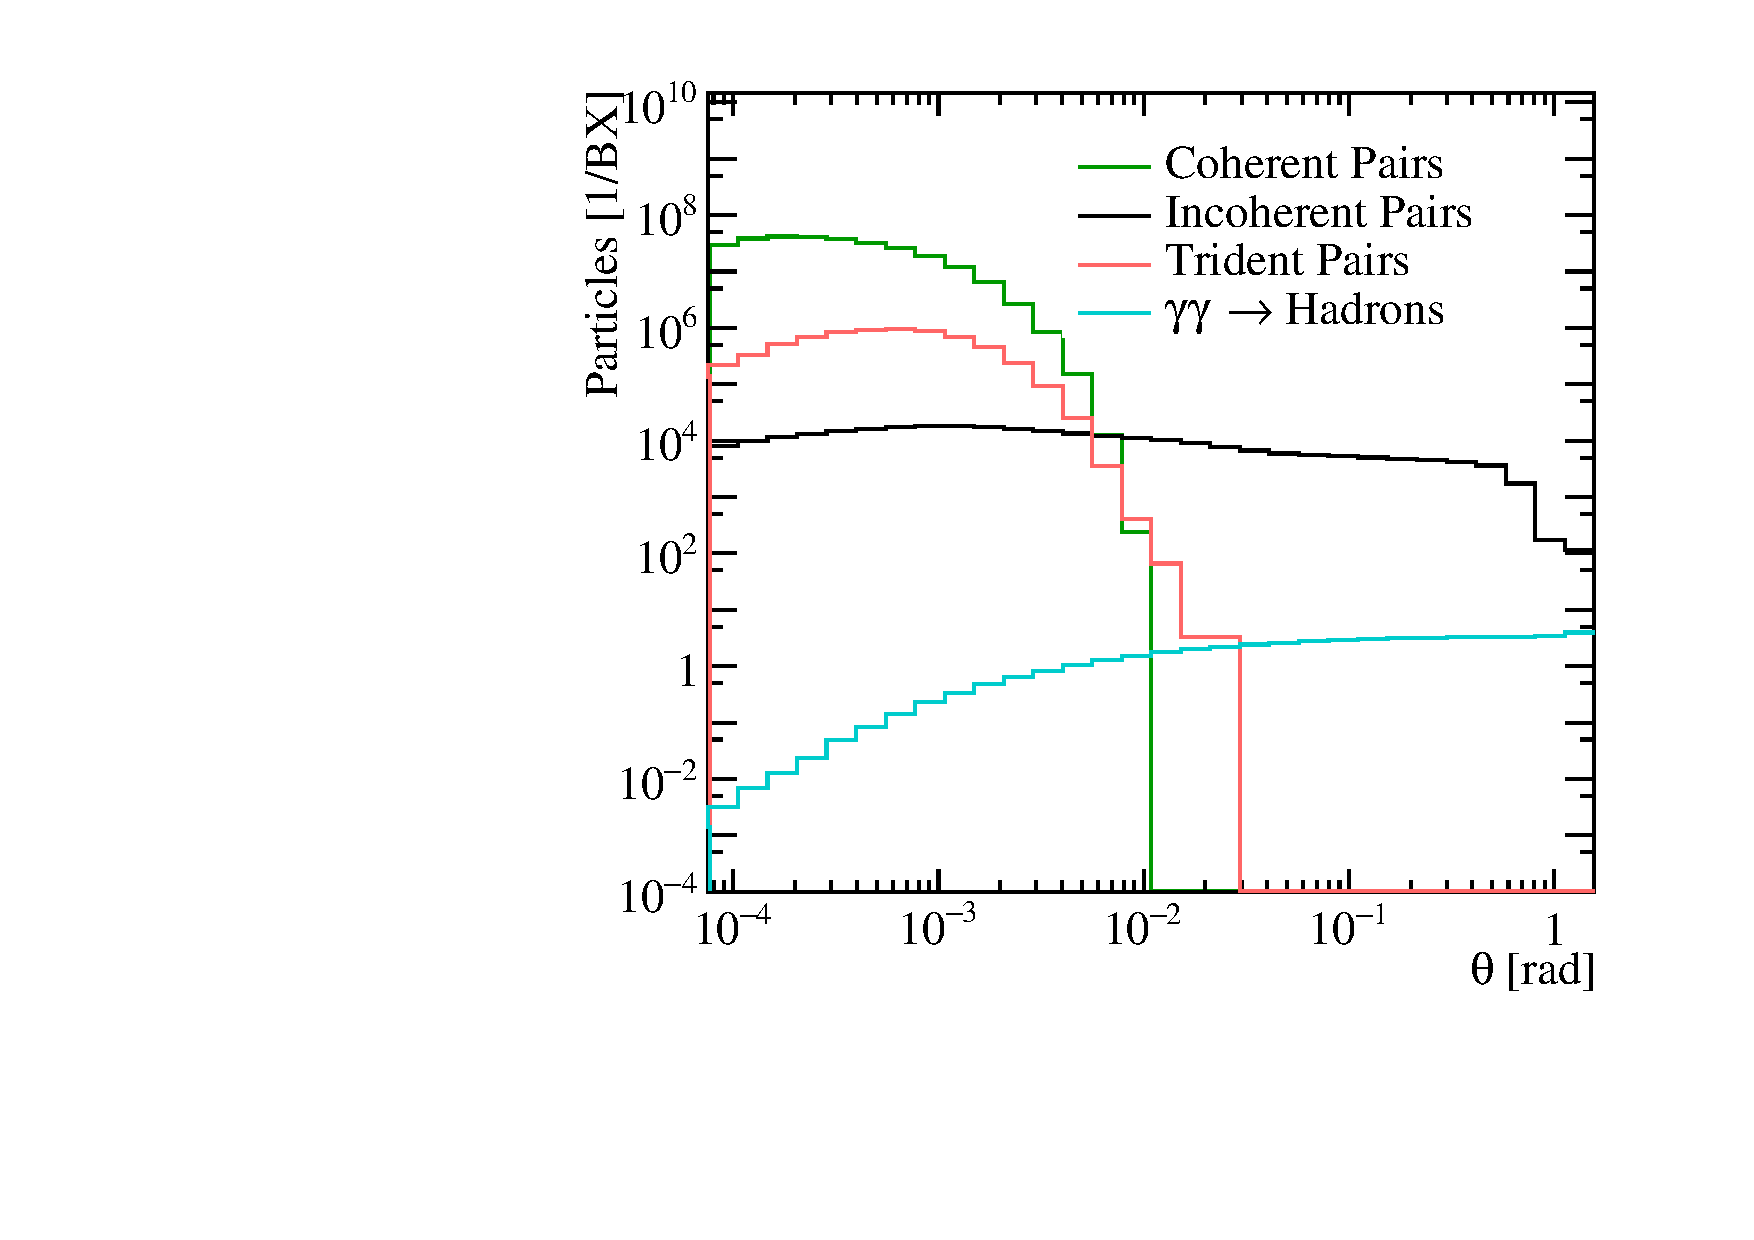
\includegraphics[width=0.5\textwidth]{FutureLinearColliders/Plots/CDRPlots/BackgroundAngleCut.pdf}
\caption[]{Angular distribution of number of particles for beam induced backgrounds for CLIC at $\sqrt{s} = 3$ TeV.  Taken from CLIC CDR.}
\label{fig:backgroundangle}
\end{figure}